\section{Bereitstellung der Biosignaldaten} \label{sec:prepdwtofhir}

Mit der Modellierung der Zuweisung der Felder und der Definition von neuen Transformationsregeln für die Überführung der Biosignaldaten aus \ac{copra} in die \ac{fhir}-Ressourcen des Moduls \glqq Intensivmedizin\grqq{} wurden drei \ac{sql}-Views programmiert, um die Elemente der Profile, die Attribute der Biosignaldaten in den Werttabellen, zusammen mit den dazugehörigen Daten der behandelten Personen, zu verlinken und zu visualisieren. Die angelegten \ac{sql}-Views sind Folgende:

\begin{itemize}
	\item \texttt{v\_profil\_decimal}: Information der Profile und der Biosignaldaten in der Tabelle \texttt{co6\_data\_decimal\_6\_3}
	\item \texttt{v\_profil\_string}: Information der Profile und der Biosignaldaten in der Tabelle \texttt{co6\_data\_string}
    \item \texttt{v\_profil\_pressure}: Information der Profile und der Biosignaldaten in der Tabelle \texttt{co6\_medic\_pressure}
\end{itemize}

Der Inhalt der Spalten der \ac{sql}-Views sind die spezifizierten Parameter der Tabellen in der Subsektion \ref{subsec:modellinksystems}. 
\newpage
Der Code \ref{list:viewpressure} zeigt den \ac{sql}-Befehl für die Erzeugung der \ac{sql}-View für die Bioparameter in der Tabelle \texttt{co6\_data\_string}. 

\begin{lstlisting}[language=SQL, caption={[SQL-View für Werte in co6\_data\_string] SQL-View für Werte in co6\_data\_string.}, captionpos=b, label=list:viewsdicimalstring]
	create or replace view copra.v_profil_string 
	as
	  select 
        's_'||md5(
	      (select table_name 
	      from information_schema.tables 
	      where table_schema = 'copra'
	      and table_name = 'co6_data_string') 
	      || cdd.id 
	      || mmc.profile_name) id, -- ID aus der Zusammensetzung vom Namen der Werttabelle, id des Werts und Name des Profils
	    mmc.meta_profile,
	    'final' status,
	    mmc.category_coding_system,
	    mmc.category_coding_code,
	    mmc.code_coding_system_snomed,
	    mmc.code_coding_code_snomed,
      mmc.code_coding_system_loinc,
      mmc.code_coding_code_loinc,
      mmc.code_coding_system_ieee,
      mmc.code_coding_code_ieee,
		 'p_'||md5(cmdp.id::varchar) subject_reference,
		 cdd.val::decimal * mmc.unit_transform "valueQuantity_value",  -- type casting und Umrechnung
      mmc.valuequantity_system "valueQuantity_system",
      mmc.valuequantity_code "valueQuantity_code",
		  cdd.datetimeto "effectiveDataTime"
	from copra.co6_data_string cdd 
	join copra.co6_config_variables ccv 
	  on cdd.varid = ccv.id 
	join copra.mapping_mii_co6_2 mmc 
	  on mmc.conf_var_id = ccv.id 
	join copra.co6_medic_data_patient cmdp 
	  on cmdp.id = cdd.parent_id 
	where not cdd.deleted
	and cdd.validated 
	and cdd.flagcurrent
	and cdd.val ~ '^\d+$|^\d+\.\d+$' -- Kontrolle der nummerischen Struktur der Werte
	;
\end{lstlisting}

\newpage

Ein Screenshot von einigen der Spalten der \ac{sql}-View \texttt{v\_profil\_string} ist in der \ref{fig:viewstring} zu sehen.

\begin{figure}[ht]
	\centering
	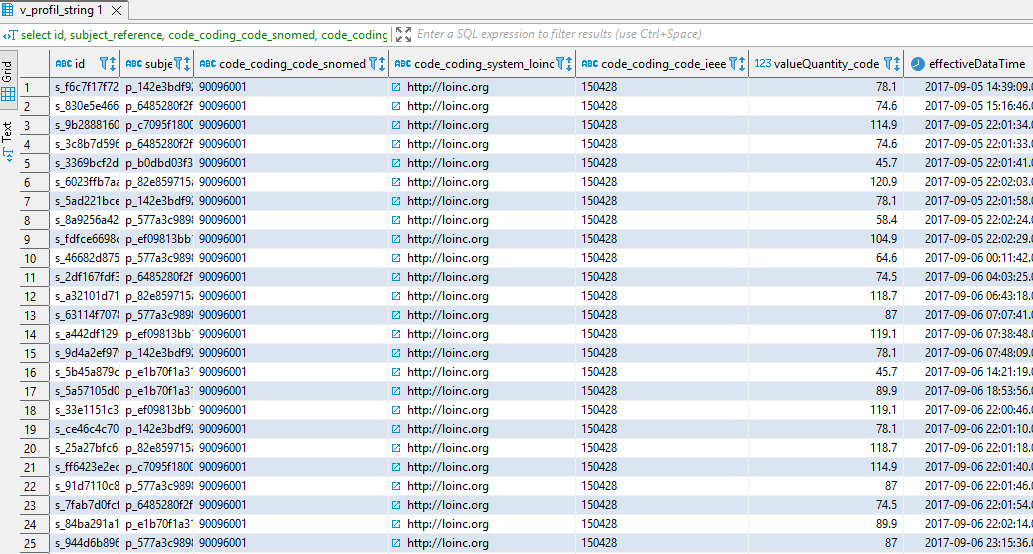
\includegraphics[width=1\textwidth]{figures/view_string}
	\caption[Screenshot der \acs{sql}-View \texttt{co6\_data\_string}]{Screenshot der \acs{sql}-View \texttt{co6\_data\_string}.}
	\label{fig:viewstring}
\end{figure}

Die \ac{sql}-View für die Biosignale in \texttt{co6\_data\_decimal\_6\_3} wird in dieser Arbeit nicht präsentiert, denn diese View ist ähnlich wie die View für die String-Werte, aber weniger komplex. Der Grund hierzu ist, dass die detektierten Biosignaldaten in \texttt{co6\_data\_string}, die den \ac{fhir}-Profilen zugeordnet sind, in Wahrheit numerische Einträge sind (\ref{tab:stringvalue}), und somit sollte der Datentyp dieser Biosignaldaten umgewandelt werden, jedoch muss zuvor die Struktur des Wertes in der Spalte \texttt{val} der Tabelle \texttt{co6\_data\_string} kontrolliert werden (\ref{sec:transfer}).

\begin{table}[ht]
	\centering 
	\caption[Eintrag in der Tabelle co6\_data\_string]{Beispiel eines Eintrags in der Tabelle co6\_data\_string. Der angezeigte Wert des Biosignals ist eine Zahl.}
	\label{tab:stringvalue}
	\begin{tabular}{|l|l|l|}
		\hline
		\bfseries Profil & \bfseries Konfigurationsvariable & \bfseries Wert \\ \hline
		Linksventrikulaeres Schlagvolumen & SV & 78.1 \\ \hline
	\end{tabular}
\end{table}

In der \ac{sql}-View für die Blutdruckwerte (Code \ref{list:viewpressure}) werden die Suffixe \glqq systolic\grqq{} für systolisch, \glqq mean\grqq{} für mittel und \glqq diastolic\grqq{} für diastolisch angewendet, um die Zusammensetzung dieser Werte in den zugeordneten \ac{fhir}-Profilen darzustellen (\ref{sec:fhirprofs}). 

\begin{lstlisting}[language=SQL, caption={[SQL-View für Werte in co6\_medic\_pressure] SQL-View für Werte in co6\_medic\_pressure.} , captionpos=b, label=list:viewpressure]
create or replace view copra.v_profil_pressure 
as
	select 
		'pr_'||md5(
			(select table_name 
			from information_schema.tables 
			where table_schema = 'copra'
			and table_name = 'co6_medic_pressure') 
			|| cdd.id 
			|| mmc.profile_name) id,
		mmc.meta_profile,
		'final' status,
		mmc.category_coding_system,
		mmc.category_coding_code,  
		'p_'||md5(cmdp.id::varchar) subject_reference,
		cdd.datetimeto "effectiveDataTime",
		mmc.code_systolic_coding_system_snomed,
		mmc.code_systolic_coding_code_snomed,
		mmc.code_systolic_coding_system_loinc,
		mmc.code_systolic_coding_code_loinc,
		mmc.code_systolic_coding_system_ieee,
		mmc.code_systolic_coding_code_ieee,
		cdd.systolic "valueQuantity_value_systolic",
		mmc.valuequantity_system "valueQuantity_system_systolic",
		mmc.valuequantity_code "valueQuantity_code_systolic",
		mmc.code_mean_coding_system_snomed,
		mmc.code_mean_coding_code_snomed,
		mmc.code_mean_coding_system_loinc,
		mmc.code_mean_coding_code_loinc,
		mmc.code_mean_coding_system_ieee,
		mmc.code_mean_coding_code_ieee,
		cdd.mean "valueQuantity_value_mean",
		mmc.valuequantity_system "valueQuantity_system_mean",
		mmc.valuequantity_code "valueQuantity_code_mean",
		mmc.code_diastolic_coding_system_snomed,
		mmc.code_diastolic_coding_code_snomed,
		mmc.code_diastolic_coding_system_loinc,
		mmc.code_diastolic_coding_code_loinc,
		mmc.code_diastolic_coding_system_ieee,
		mmc.code_diastolic_coding_code_ieee,
		cdd.mean "valueQuantity_value_diastolic",
		mmc.valuequantity_system "valueQuantity_system_diastolic",
		mmc.valuequantity_code "valueQuantity_code_diastolic"
	from copra.co6_medic_pressure cdd 
	join copra.co6_config_variables ccv 
		on cdd.varid = ccv.id 
	join copra.mapping_mii_co6_2 mmc 
		on mmc.conf_var_id = ccv.id 
	join copra.co6_medic_data_patient cmdp 
		on cmdp.id = cdd.parent_id 
	where cdd.validated 
	and not cdd.deleted 
	and cdd.flagcurrent
;
\end{lstlisting}

Mit diesen \ac{sql}-Views können \ac{fhir}-Ressourcen wie im Code \ref{list:fhirres} erzeugt werden, denn eine Zeile in der View entspricht einer \ac{fhir}-Ressource im Modul \glqq Intensivmedizin\grqq{}.

\begin{lstlisting}[caption={[Beispiel einer \acs{fhir}-Ressource aus \acs{copra}] Beispiel einer \acs{fhir}-Ressource einer Blutdruckmessung aus \acs{copra}.},language=JavaScript, label=list:fhirres, captionpos=b]
	{
		"resourceType": "Observation",
		"id": "pr_d43de0fb06ce5b34d7692ad69b59771f",
		"meta": {
			"profile":  [
			"https://medizininformatik-initiative.de/fhir/ext/modul-icu/
			StructureDefinition/pulmonalarterieller-blutdruck"
			]
		},
		"status": "final",
		"category":  [
		{
			"coding":  [
			{
				"system": "http://terminology.hl7.org/
				CodeSystem/observation-category",
				"code": "vital-signs"
			}
			]
		}
		],
		"code": {
			"coding":  [
			{
				"system": "http://snomed.info/sct",
				"code": "75367002",
			}
			]
		},
		"subject": {
			"reference": "p_e139c454239bfde741e893edb46a06cc"
		},
		"effectiveDateTime": "2022-11-25T09:30:11+01:00",
		"component":  [
		{
			"code": {
				"coding":  [
				{
					"system": "http://loinc.org",
					"code": "8406-1"
				},
				{
					"system": "urn:iso:std:iso:11073:10101",
					"code": "150107"
				}
				]
			},
			"valueQuantity": {
				"value": 104,
				"system": "http://unitsofmeasure.org",
				"code": "mm[Hg]"
			}
		},
		{
			"code": {
				"coding":  [
				{
					"system": "http://loinc.org",
					"code": "8432-7"
				},
				{
					"system": "urn:iso:std:iso:11073:10101",
					"code": "150105"
				}
				]
			},
			"valueQuantity": {
				"value": 86,
				"system": "http://unitsofmeasure.org",
				"code": "mm[Hg]"
			}
		},
		{
			"code": {
				"coding":  [
				{
					"system": "http://loinc.org",
					"code": "8377-4"
				},
				{
					"system": "urn:iso:std:iso:11073:10101",
					"code": "150106"
				}
				]
			},
			"valueQuantity": {
				"value": 67,
				"system": "http://unitsofmeasure.org",
				"code": "mm[Hg]"
			}
		}
		]
	}
\end{lstlisting}